\documentclass[12pt,a4paper]{report}
\usepackage[utf8]{inputenc}
\usepackage[inner=3.5cm,outer=2.5cm,bottom=3cm,top=2.5cm,pdftex]{geometry}
\usepackage{setspace}
\usepackage{graphicx}
\usepackage{rotating}
\usepackage[page]{appendix}
\usepackage{float}
\usepackage[font=small,labelfont=bf]{caption}
\usepackage{subfigure}
\usepackage{titlesec}
\usepackage[hidelinks]{hyperref}
\usepackage{listings}
\usepackage{textcomp}
\usepackage{fancyhdr}
\usepackage{multirow}
\usepackage{verbatim}	%makes it possible to comment out a section of text by using \begin{comment}...\end{comment}
\usepackage[table,xcdraw]{xcolor}
\usepackage{pifont}
\usepackage{mathptmx}
\usepackage{wrapfig}
\usepackage{ragged2e}
\usepackage[nottoc,notlot,notlof]{tocbibind}
\usepackage[norsk]{babel}

\definecolor{rockwoolcolor}{RGB}{155,0,0}

% Style chapter headings for preface and toc.
\setlength{\headheight}{15pt}
\titlespacing*{\chapter}{0pt}{0pt}{4ex}
\titleformat{\chapter}[display]
 {\bfseries\Large}
 {}
 {0pt}
 {\color{rockwoolcolor}\titlerule[2.0pt]\vspace{2ex}\filright\color{black}}
 [\color{rockwoolcolor}\vspace{2ex}{\titlerule[2.0pt]}]


\setstretch{1.25}
\begin{document}
{\RaggedRight
\pagestyle{fancy}

% empty default settings for fancy layout
\fancyhf{}

% table mark commands
\newcommand{\cmark}{\textcolor{green!80!black}{\ding{51}}}
\newcommand{\xmark}{\textcolor{red}{\ding{55}}}
\newcommand{\plusmark}{\textcolor{green!80!black}{\textbf{+}}}
\newcommand{\minusmark}{\textcolor{red}{\textbf{-}}}

% chapter, section, header and footer layout
\renewcommand{\sectionmark}[1]{\markright{\thesection ~ \ #1}}
\renewcommand{\chaptermark}[1]{\markboth{ #1}{}}
\renewcommand{\headrulewidth}{0.5pt}
\renewcommand{\footrulewidth}{0.5pt}

%head setting
\fancyhead[L]{\textcolor{black} {\rightmark}}
\fancyfoot[C]{\textcolor{black} {\thepage}}

% Redefine the plain page style - used when the page is a chapter
\fancypagestyle{plain}{%
  \fancyhf{}%
  \renewcommand{\headrulewidth}{0pt}% Line at the header invisible
  \renewcommand{\footrulewidth}{0.5pt}% Line at the footer visible
  \fancyfoot[C]{\textcolor{black} {\thepage}}
}

% Avoid hyphenating
\tolerance=10
\emergencystretch=\maxdimen
\hyphenpenalty=10000
\hbadness=10000

\pagenumbering{roman}
\chapter*{Executive Summary}
\textit{ROCKWOOL bør utvikle seg mot en grønn fremtid.}

\indent \newline
AS ROCKWOOL (heretter omtalt som ROCKWOOL) er et heleid norsk datterselskap av ROCKWOOL international A/S. ROCKWOOL er en isolasjonsprodusent som baserer sin virksomhet på utvinning av vulkansk stein. Visjonen deres er \textit{\textquotedblleft AS ROCKWOOL skal være ledende leverandør av isolasjon, der positivt bidrag til et bedre miljø og brannsikring skal være førende.\textquotedblright} Bedriften har i flere år levert gode resultater, og er markedets nest største aktør. Den siste tiden har de imidlertid opplevd en lavere prosentvis vekst, grunnet en utvikling i markedet hvor miljøet blir vektlagt mer enn tidligere.

\indent \newline
De interne analysene viser at ROCKWOOL har flere sterke og svake sider. Med en markedsandel på ca 26\%, oppnår bedriften stordriftsfordeler som gir lavere enhetskostnader. Gjennom Ropex fokuseres det kontinuerlig på effektivisering av verdikjeden. De har i utgangspunktet konkurransefortrinn i produktegenskapene, men klarer ikke å utnytte dette godt nok. Årsaken er nåværende produksjonsteknologi som gir et høyere CO2-utslipp enn de nærmeste konkurrentene. En annen svak side er høye transportkostnader grunnet komprimeringsegenskapene til produktet. Analysene viser videre at bedriften besitter høy kompetanse, i form av erfaring og lav turnover. Bedriften bør imidlertid være oppmerksom på en høy gjennomsnittsalder blant de ansatte. 

\indent \newline
Resultatene fra de eksterne analysene viser til en høy forhandlingsmakt hos kundene. En økende bruk av BREEAM-sertifisering blant entreprenørene fører til strengere produktkrav i form av lavt CO2-utslipp. Bransjeanalysen viser til et modent marked med lav vekst, og består av noen få store aktører. Konkurranseintensiteten anses som høy og vedvarende. 

\indent \newline
Basert på analysene har jeg identifisert fire strategiske handlingsalternativer som kan hjelpe ROCKWOOL med å nå sin visjon:

\begin{itemize}
\item[1.]\textbf{Fortsette med organisk vekst}
\indent \newline
Fokus på organisk vekst har så langt blitt vektlagt av ROCKWOOL. Flere år med solide økonomiske tall gjør det naturlig å fortsette med samme strategi. En godt innarbeidet Lean-metode (Ropex) og interne opplærings- og utdanningssystemer gjør ROCKWOOL til en veldreven og kostnadseffektiv bedrift. Fremtidige fokusområder bør være teknologiutvikling relatert til produktkomprimering og bevaring av kompetanse. 

\item[2.]\textbf{Go Green}
\indent \newline
Implementere en miljøvennlig profil gjennom hele verdisystemet. Investering i en fullskala el-ovn vil kunne redusere CO2-utslippet med ca. 80\% og gjøre ROCKWOOL til en foretrukken leverandør blant entreprenørene. På sikt bør bedriftens inngående- og utgående logistikk bestå av leverandører som benytter el-transport.

\item[3.]\textbf{Oppkjøp/Fusjon}
\indent \newline
Oppkjøp eller fusjon er en rask måte for ROCKWOOL å utvide markedsandelen sin på. Paroc anses som en potensiell kandidat med tanke på integrasjonsprosessen og koordinering av aktiviteter. Valget vil gi økte stordriftsfordeler og lavere enhetskostnader, og tilgang til andre operasjonelle synergier.

\item[4.]\textbf{Geografisk utvidelse}
\indent \newline
En fabrikkutvidelse i Sverige vil kunne øke omsetningen i det svenske markedet gjennom nærhet til markedet og reduserte transportkostnader.
\end{itemize}
\indent
Det presiseres at alternativ tre og fire vil være strategier som ROCKWOOL må bringe videre til konsernledelsen for håndtering og godkjenning.

\indent \newline
Basert på analysene mener jeg en kombinasjon av handlingsalternativene “Fortsette med organisk vekst” og “Go Green” vil kunne hjelpe ROCKWOOL med å nå sin visjon. Den anbefalte løsningen samsvarer med markedsutviklingen og de største truslene bedriften står overfor i dag. Ved å kombinere nåværende strategi med en grønn utvikling vil de kunne bli en foretrukket leverandør blant entreprenørene, og dermed utvide markedsandelen på sikt. Investering i en ny el-smelteovn vil være bedriftsøkonomisk ulønnsom de første årene, grunnet en prøveperiode med implementering av teknologien. Investeringen vil kreve betydelige finansielle midler og det anbefales derfor å søke om støtte fra Enova. Ved avslag må finansiell støtte hentes fra ROCKWOOL international A/S. 

\indent \newline
Link til video: 


\setcounter{tocdepth}{2}
\tableofcontents
\addtocontents{toc}{~\hfill\textbf{Side}\par}

% ----------- CHAPTERS ----------------

% Parts
\cleardoublepage
% Style chapter headings.
\titleformat{\chapter}[display]
 {\bfseries\Large}
 {}
 {0pt}
 {\color{rockwoolcolor}\titlerule[2.0pt]\vspace{2ex}\filright\color{black} \thechapter . }
 [\color{rockwoolcolor}\vspace{2ex}{\titlerule[2.0pt]}]
\pagenumbering{arabic}
\setcounter{page}{1}
\chapter{Bedriften AS ROCKWOOL}
\input{kapittel/bedriftenAsRockwool}

\chapter{Intern analyse}
\section{Verdikonfigurasjons-analyse}
Verdikonfigurasjonsanalysen identifiserer sammensetningen av bedriftens aktiviteter og tilhørende verdi- og kostnadsdrivere \cite[s.~32]{FjeldstadogLunnan2018}. AS ROCKWOOL driver med industriell produksjon som er typisk for en verdikjede.

\begin{figure}[H]
\centering
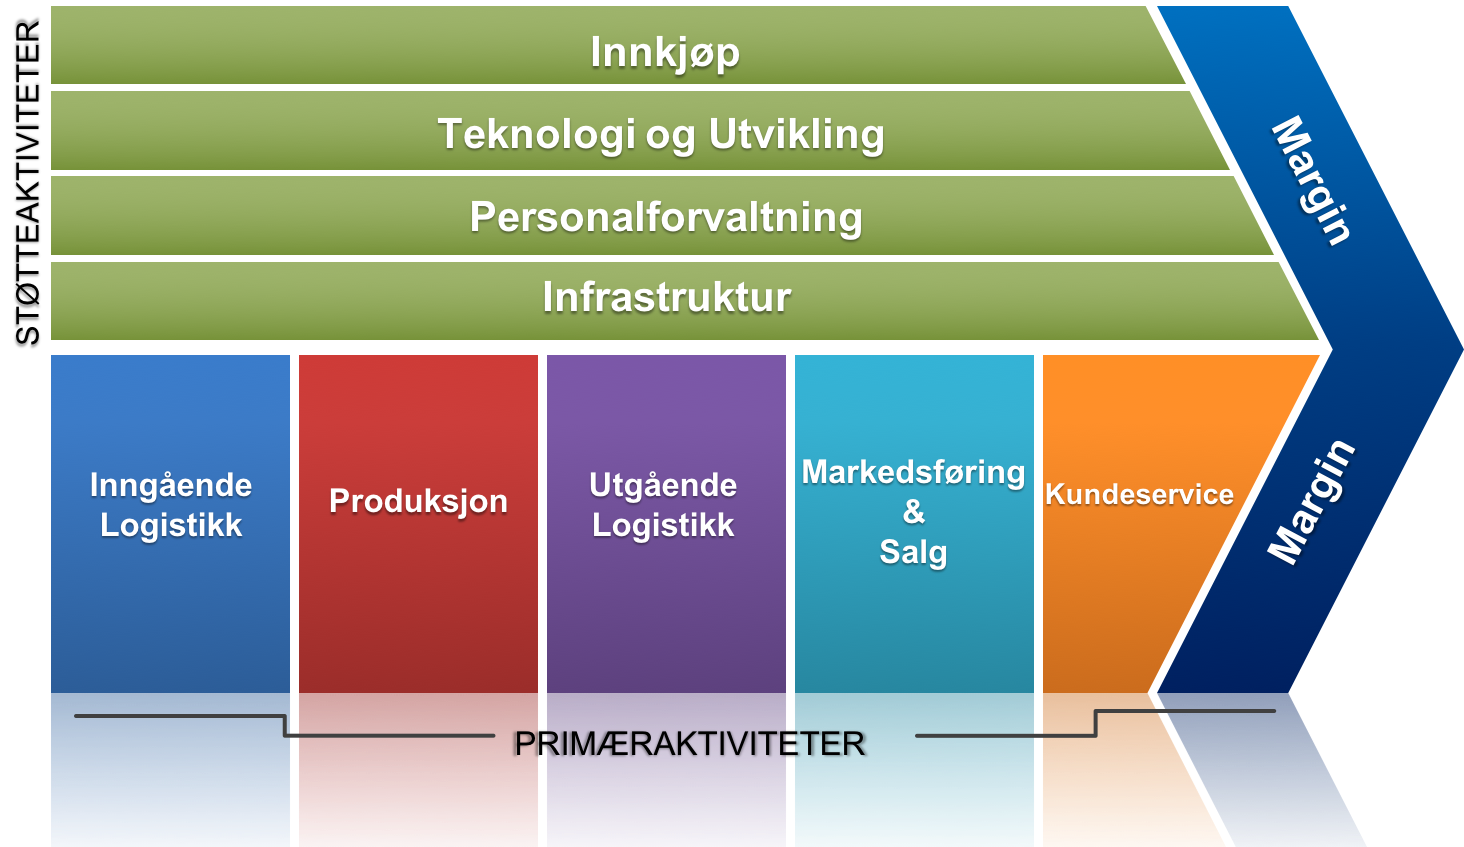
\includegraphics [scale=0.5]{bilder/verdikjede.png}
\caption{ROCKWOOL verdikjede}
\label{fig:verdikjede}
\end{figure}

\subsection{Primæraktiviteter}
Primæraktivitene er et sekvensielt sett av aktiviteter som direkte skaper verdi for kunden \cite[s.~132]{FjeldstadogLunnan2018}. 
 
\indent \newline
Som vist i figur \ref{fig:verdikjede} er den første aktiviteten inngående logistikk. Råvarer som vulkansk stein, koks og slagg (avfallsprodukter fra aluminiumsproduksjon) lagres, før det fraktes videre til produksjon. Her omformes innsatsfaktorene fra råvarer til steinull ved å bli utsatt for enormt høye temperaturer i en smelteovn. De ferdige produktene fraktes videre til lagring eller transporteres direkte til kunder avhengig av om det er produsert på bestilling. Markedsføring og salg fokuserer på byggevarekjeder og entreprenører. Det markedsføres derfor ikke direkte mot privatpersoner. Kundeservice består i hovedsak av teknisk service.

\indent \newline
ROCKWOOL har utfordringer med høye transportkostnader i forhold til andre konkurrenter grunnet hvor godt produktene lar seg komprimere. Produktene transporteres med lastebil ved fastprisavtale, og dårligere komprimering av produktene gir dermed lavere volum per transport. 

\subsection{Støtteaktiviteter}
Støtteaktivitetene skaper indirekte verdi for kunden gjennom sin effekt på primæraktivitetene \cite[s.~132]{FjeldstadogLunnan2018}. 

\subsubsection*{Innkjøp}
ROCKWOOL oppnår fordelaktige innkjøpsavtaler gjennom sin størrelse og store innkjøpskvantum, og blir videre forsterket gjennom sentral koordinering fra sitt konsern.

\subsubsection*{Teknologi og utvikling}
Både i AS ROCKWOOL og konsernet har de i mange år lagt mye ressurser i teknologiutvikling. De har tidligere utviklet sitt eget bindemiddel som gir energieffektiv og lydreduserende isolasjon, og dermed et konkurransedyktig produkt. I dag jobbes det med å forbedre komprimeringsegenskapene for å redusere kostnadene forbundet med transport.

\subsubsection*{Personalforvaltning}
De ansatte trives godt i jobben og føler tilhørighet til arbeidsoppgavene. Det er innarbeidet gode rutiner som sørger for at det er to personer med samme kompetanse til å utføre hver arbeidsoppgave. Dette sørger for en kontinuerlig flyt selv ved sykefravær og eventuelle oppsigelser.

\subsubsection*{Infrastruktur}
Vedlikehold og drift av produksjonen vurderes regelmessig etter KPIer (Key Performance Indicators). Dette er viktige nøkkeltall som ledelsen bruker for å evaluere måloppnåelse. Ledelsen har også tatt i bruk en Lean-metode som de kaller for Ropex. Metoden sørger for et kontinuerlig fokus på effektivitetsforbedringer.

\subsubsection*{Oppsummering}
ROCWOOL har i flere år jobbet med å effektivisere verdikjeden. Gjennom implementering av Ropex har bedriften tilegnet seg god kommunikasjon på tvers av avdelinger og kommandolinjer med fokus på å produsere mest mulig effektivt. På bakgrunn av dette, ser man lite rom for forbedring i verdikjeden. Det ligger imidlertid forbedringspotensial innenfor teknologiutvikling for å kunne forbedre kompaktheten til produktene og dermed øke volumet per transport.

\section{Verdikjedens drivere}
Verdikjedens drivere er strukturelle faktorer som påvirker verdiskapning for kunden og enhetskostnadene forbundet med å utføre aktivitetene \cite[s.~32]{FjeldstadogLunnan2018}. De viktigste driverne for ROCKWOOL er stordriftsfordeler og kapasitetsutnyttelse. Bedriften kan lagre produktene i opp til ett år før de må gjennom en ny kvalitetskontroll. Lang holdbarhet på produktene gir mulighet til å produsere i stor skala og dermed senke enhetskostnadene. Stordriftsfordelene forsterkes også av å være en del av ROCKWOOL-konsernet. Bedriften drar nytte av operasjonelle synergier gjennom gunstige prisavtaler hos leverandører ved å handle i stort kvantum.

\section{VRIO-analyse}
\begin{table}[ht]
\centering
\resizebox{\textwidth}{!}{%
\begin{tabular}{lccccc}
\hline
\rowcolor[HTML]{656565} 
{\color[HTML]{FFFFFF} \textbf{Ressurs}}                                                          & {\color[HTML]{FFFFFF} \textbf{Verdifull}} & {\color[HTML]{FFFFFF} \textbf{Sjelden}} & {\color[HTML]{FFFFFF} \textbf{Vanskelig å kopiere}} & {\color[HTML]{FFFFFF} \textbf{Effektivt organisert}} & {\color[HTML]{FFFFFF} \textbf{Avkastning}}     \\ \hline
\multicolumn{1}{|l|}{\cellcolor[HTML]{9B0000}{\color[HTML]{FFFFFF} \textbf{Finansiell kapital}}} & \multicolumn{1}{c|}{\cmark}                   & \multicolumn{1}{c|}{\xmark}                & \multicolumn{1}{c|}{\xmark}                            & \multicolumn{1}{c|}{\cmark}                              & \multicolumn{1}{c|}{\footnotesize Over gjennomsnittet}       \\ \hline
\multicolumn{1}{|l|}{\cellcolor[HTML]{9B0000}{\color[HTML]{FFFFFF} \textbf{Kompetanse}}}         & \multicolumn{1}{c|}{\cmark}                   & \multicolumn{1}{c|}{\cmark}                 & \multicolumn{1}{c|}{\cmark}                             & \multicolumn{1}{c|}{\cmark}                              & \multicolumn{1}{c|}{\footnotesize Over gjennomsnittet}       \\ \hline
\multicolumn{1}{|l|}{\cellcolor[HTML]{9B0000}{\color[HTML]{FFFFFF} \textbf{Teknologi}}}          & \multicolumn{1}{c|}{\cmark}                   & \multicolumn{1}{c|}{\xmark}                & \multicolumn{1}{c|}{\xmark}                            & \multicolumn{1}{c|}{\xmark}                             & \multicolumn{1}{c|}{\footnotesize Litt under gjennomsnittet} \\ \hline
\multicolumn{1}{|l|}{\cellcolor[HTML]{9B0000}{\color[HTML]{FFFFFF} \textbf{Produktegenskaper}}}  & \multicolumn{1}{c|}{\cmark}                   & \multicolumn{1}{c|}{\xmark}                & \multicolumn{1}{c|}{\cmark}                             & \multicolumn{1}{c|}{\cmark}                              & \multicolumn{1}{c|}{\footnotesize Over gjennomsnittet}       \\ \hline
\end{tabular}%
}
\caption{Ressursanalyse}
\label{ressursanalyse}
\end{table}

\subsection{Finansiell kapital}
ROCKWOOL har hatt en lønnsom drift i flere år og hadde i 2017 et årsresultat på 64 millioner kroner og en egenkapital på 382 millioner kroner \cite{ProffRegnskap}. I tillegg drar de nytte av finansielle synergier ved å være en del av et konsern. De står dermed godt rustet for potensielle investeringer i tiden fremover.

\subsection{Kompetanse}
Kompetansen anses som meget god. Turnover-raten er på bare 2\% og mange av de ansatte har en fartstid på 15-35 år i bedriften. For å fortsette kompetanseutviklingen blant de ansatte har de innarbeidet interne opplærings- og utdanningssystemer. Bedriften bør imidlertid være oppmerksom på at kompetanse kan forsvinne i årene som kommer på grunn av en relativt høy gjennomsnittsalder.

\subsection{Teknologi}
Det investeres mye ressurser i teknologi, både i ROCKWOOL og konsernet. Utvikling av egne smelteovner har tidligere gitt konkurransefortrinn i markedet, men med dagens smelteteknologi henger de etter de største konkurrentene med tanke på å produsere miljøvennlig. Å redusere CO2-utslipp i forbindelse med produksjonsprosessen anses som kritisk for å kunne være konkurransedyktige i fremtiden.

\subsection{Produktegenskaper}
Steinull innehar flere egenskaper og bruksområder enn de fleste andre isolasjonsproduktene i markedet. Produktet isolerer, er vannavstøtende, har lyddempende egenskaper og er en god kilde til brannsikring. Det er kun ROCKWOOL og Paroc som scorer høyt på alle disse produktattributtene, mens andre aktører kun leverer på to av punktene.

\subsection{Oppsummering}
Analysen viser at ROCKWOOL har konkurransefortrinn i produktegenskapene. Dette anses som langvarig da egenskapene kommer naturlig fra råvaren i kombinasjon med et egetutviklet bindemiddel. Det vil også være kostbart for andre aktører å bytte til steinullproduksjon i form av store investeringer og mangel på erfaring. Fremover vil det være viktig å utvikle og investere i ny miljøvennlig smelteteknologi som jeg anser som en av bedriftens største utfordringer i dag.

\chapter{Ekstern analyse}
Denne seksjonen tar for seg Porters fem krefter og PESTEL- analyse, som gir innsikt i byggisolasjonsbransjen og bedriftens makroomgivelser. Analysene kartlegger eventuelle trusler og muligheter bedriften står overfor i tiden fremover.

\section{Konkurransearena}
\begin{wrapfigure}{l}{0.5\textwidth}
  \begin{center}
    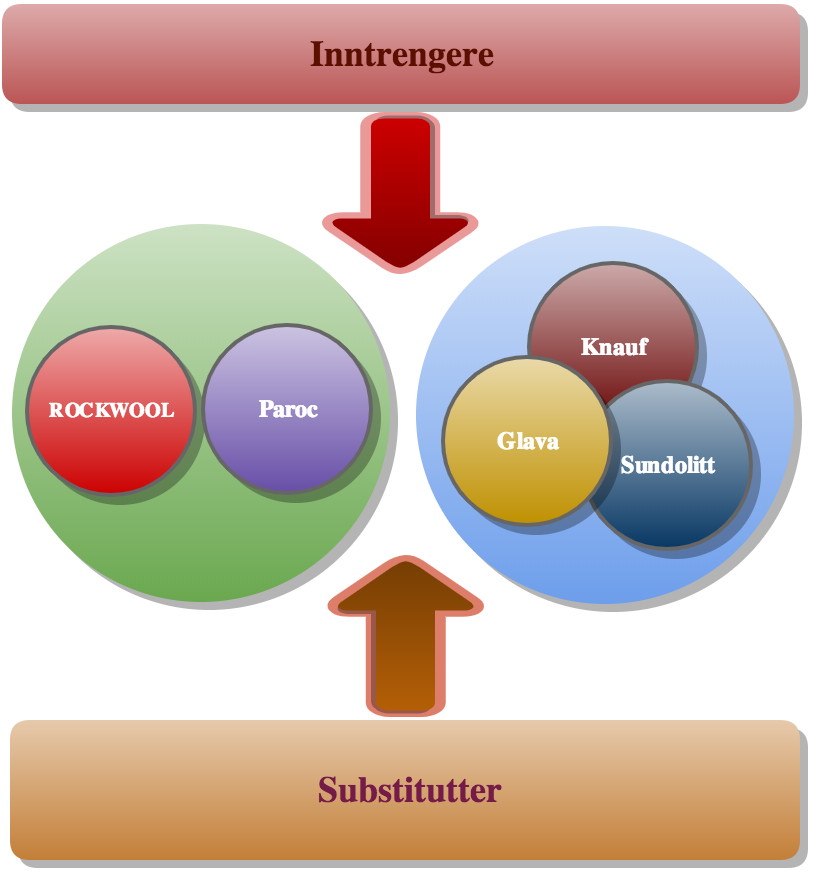
\includegraphics[width=0.48\textwidth, scale=0.2]{bilder/strategiskeGrupper.png}
  \end{center}
  \caption{Strategiske grupper}
  \label{fig:strategiskeGrupper}
\end{wrapfigure}

\indent \newline
ROCKWOOL sin konkurransearena er byggisolasjon, og er avgrenset til det norske og svenske markedet som bedriften leverer til.  Konkurrenter er henholdsvis de samme i både Norge og Sverige, hvor Glava, Knauf, Sundolitt og Paroc er de største. Glava produserer glassullisolasjon og har størst markedsandel på 40\%. Paroc er ROCKWOOL sin mest nærliggende konkurrent da de produserer steinullisolasjon. De siste årene har det kommet nye alternative isolasjonsprodukter som halmtekstil, papir og trefiber.

\indent \newline
\indent \newline
\begin{table}[ht]
\centering
\resizebox{\textwidth}{!}{%
\begin{tabular}{|l|c|c|c|c|c|}
\hline
\rowcolor[HTML]{656565} 
{\color[HTML]{FFFFFF} \textbf{Bedrift}}                          & {\color[HTML]{FFFFFF} \textbf{Råvare}} & {\color[HTML]{FFFFFF} \textbf{Isolasjon}} & {\color[HTML]{FFFFFF} \textbf{Vannavstøtende}} & {\color[HTML]{FFFFFF} \textbf{Lydisolasjon}} & {\color[HTML]{FFFFFF} \textbf{Brannsikring}} \\ \hline
\cellcolor[HTML]{FFFFFF}{\color[HTML]{000000} \textbf{ROCKWOOL}} & Steinull                               & \plusmark                                         & \plusmark                                              & \plusmark                                            & \plusmark                                            \\ \hline
\cellcolor[HTML]{FFFFFF}{\color[HTML]{000000} \textbf{Paroc}}    & Steinull                               & \plusmark                                         & \plusmark                                              & \plusmark                                            & \plusmark                                            \\ \hline
\cellcolor[HTML]{FFFFFF}{\color[HTML]{000000} \textbf{Glava}}    & Glassull                               & \plusmark                                         & \minusmark                                              & \minusmark                                            & \plusmark                                            \\ \hline
\cellcolor[HTML]{FFFFFF}{\color[HTML]{000000} \textbf{Knauf}}    & Glassull                               & \plusmark                                         & \minusmark                                              & \minusmark                                            & \plusmark                                            \\ \hline
\cellcolor[HTML]{FFFFFF}\textbf{Sundolitt}                       & Plastull                               & \plusmark                                         & \plusmark                                              & \minusmark                                            & \minusmark                                            \\ \hline
\end{tabular}%
}
\caption{Produktegenskaper}
\label{produktegenskaper}
\end{table}
\indent \newline
Bedriftens strategiske gruppe identifiseres ved deres konkurranse og tilnærming til kunder \cite[s.~88]{FjeldstadogLunnan2018}. Samtlige aktører i markedet konkurrerer om de samme kundene, som i hovedsak er større entreprenører og byggevarekjeder. Derimot gjør produktegenskapene det naturlig å dele aktørene inn i to ulike strategigrupper. Paroc er den bedriften som likner mest, og plasseres derfor i samme gruppe som ROCKWOOL, mens Glava, Knauf og Sundolitt plasseres i en annen.
 
\section{Porters fem krefter}
\begin{figure}[H]
\centering
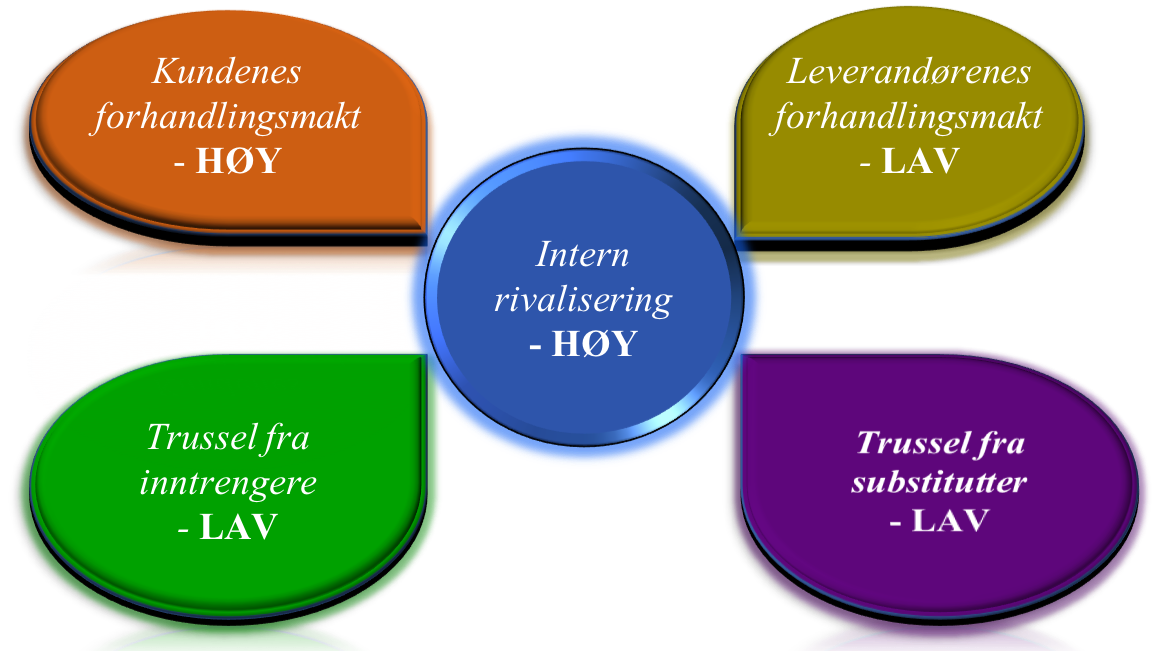
\includegraphics [scale=0.5]{bilder/portersFemKrefter.png}
\caption{Porters fem krefter - ROCKWOOL}
\label{fig:portersFemKrefter}
\end{figure}

\subsection{Trussel fra inntrengere}
Inntrengere er mulige nye konkurrenter som ønsker å etablere seg i byggisolasjonsbransjen \cite[s.~94]{FjeldstadogLunnan2018}. I en etableringsprosess for nye aktører tar man for seg mobilitetsbarrierene som påvirker inngang og utgang fra bransjen \cite[s.~90]{FjeldstadogLunnan2018}. Kapitalbehovet er stort, da det kreves store investeringer i spesialisert produksjonsutstyr. ROCKWOOL og de andre største aktørene har gjort disse investeringene over tid, noe som gir dem konkurransefortrinn overfor inntrengere. Som inntrengere må man også ta hensyn til høye faste kostnader og store avviklingsbarrierer. Stordriftsfordelene blant de største aktørene er også med på å redusere antall konkurrenter. Inngangsbarrierene er dermed høye og trussel fra inntrengere regnes som lav.

\subsection{Trussel fra substitutter}
Substituttene til ROCKWOOL er andre byggisolasjonsprodukter som dekker de samme behovene til kundene. Halm, papir og trefiber er alternative produkter, men har ikke nevneverdig markedsandel. Det vil allikevel være viktig å følge med på teknologiutviklingen som kan gjøre disse produktene mer konkurransedyktige i fremtiden.

\subsection{Kundenes forhandlingsmakt}
Bransjen består i hovedsak av to ulike kunder; byggevarekjeder og entreprenører. Byggevarekjedene fokuserer mest på pris, men langsiktige avtaler kan også forhandles frem ved bruk av bonuser og krav til å holde seminarer for byggevarekjedenes kunder. Entreprenørene fokuserer ikke bare på pris, men også hvor miljøvennlige produktene er. De står overfor strenge krav i forbindelse med totalt CO2-utslipp i byggeprosessen og vil derfor ofte favorisere produkter med lavest utslipp. Byggevarekjedene og entreprenørene er konsentrerte og har dermed høy forhandlingsmakt. Det er også relativt lite differensierte produkter som gir lave byttekostnader.

\subsection{Leverandørenes forhandlingsmakt}
Det finnes mange leverandører av råvarer i markedet, og flere av isolasjonsprodusentene handler i store kvantum. Dette gir høye byttekostnader og dermed lav forhandlingsmakt.

\subsection{Intern rivalisering}
Isolasjonsbransjen er et modent marked. De siste årene har markedsveksten ligget på ca. 2\%, og prognosene tyder på at dette vil fortsette i årene som kommer. Markedet består i hovedsak av noen få store aktører som omsetter for flere hundre millioner kroner. Produktene som tilbys er lite differensierte, bortsett fra Paroc og ROCKWOOL som tilbyr produkter med flere egenskaper. Bransjeanalysen viser til et marked med høy konkurranseintensitet hvor organisk vekst alene kan gjøre det vanskelig å utvide nåværende markedsandel. Muligheter for vekst vil derfor kunne ligge i oppkjøp eller fusjon.

\section{PESTEL-analyse}
Denne delen identifiserer faktorer i ROCKWOOL sine makroomgivelser som vil kunne påvirke bedriften i tiden fremover. Videre presenteres de viktigste funnene.

\begin{table}[ht]
\centering
\resizebox{\textwidth}{!}{%
\begin{tabular}{|l|l|l|l|l|l|}
\hline
\rowcolor[HTML]{656565} 
{\color[HTML]{FFFFFF} \textbf{Politiske}} & {\color[HTML]{FFFFFF} \textbf{Teknologiske}} & {\color[HTML]{FFFFFF} \textbf{Økonomiske}}                                     & {\color[HTML]{FFFFFF} \textbf{Miljømessige}}                      & {\color[HTML]{FFFFFF} \textbf{Sosiokulturelle}} & {\color[HTML]{FFFFFF} \textbf{Legale}} \\ \hline
- Enova                                   & - Elektrisk transport                        & \begin{tabular}[c]{@{}l@{}}- Oppgangskonjunktur\\ - Rentehevinger\end{tabular} & \begin{tabular}[c]{@{}l@{}}- Grønt skifte\\ - BREEAM\end{tabular} & - Urbanisering                                  & - CO2-avgift                           \\ \hline
\end{tabular}%
}
\caption{Makrofaktorer}
\label{Makrofaktorer}
\end{table}

\subsection{Politiske faktorer}
Enova forvalter midlene i energifondet. Formålet deres er å drive bransjene i Norge mot et lavutslippssamfunn. De tilbyr derfor økonomisk støtte til bedrifter som ønsker å velge mer energi- og klimavennlige løsninger \cite{Enova}. ROCKWOOL kan benytte seg av denne muligheten ved investering av miljøvennlige produksjonsutstyr.

\subsection{Teknologiske faktorer}
De siste årene har smelteteknologien utviklet seg fra kupolovner til el-ovner med et formål om å redusere utslipp. Bruk av elektriske lastebiler vil de neste årene bli viktig for transportselskaper. Denne utviklingen gir ROCKWOOL muligheter til å skape en mer miljøvennlig profil som samsvarer med deres visjon.

\subsection{Økonomiske faktorer}
Norsk økonomi har vært i moderat oppgangskonjunktur det siste halvannet året og forventes å gå inn i en høykonjunktur fremover. BNP økte i 2017 med 2\% og har fortsatt med en moderat vekst så langt i 2018. Arbeidsledigheten har falt og indikasjoner tyder på at den vil fortsette å synke. Dette er faktorer som reflekterer en forbedret materiell velstand, noe som er positivt for ROCKWOOL. Derimot vil årets renteheving og de planlagte rentehevingene i 2019 kunne påvirke folk sine muligheter for låneopptak og dermed virke negativt inn på nybygg-markedet \cite{SSB}.

\subsection{Miljømessige faktorer}
Samfunnet er inne i en utvikling hvor miljøet får større fokus enn tidligere. Flere entreprenører velger derfor å BREEAM-sertifisere prosjektene sine. BREEAM er et miljø-\newline sertifiseringsverktøy for bygninger \cite{BREEAM}, som skaper utfordringer for ROCKWOOL med dagens smelteteknologi. Bedriften kan stå i fare for å miste en betydelig markedsandel hvis de ikke tar hensyn til utviklingen.

\subsection{Sosiokulturelle faktorer} 
På bakgrunn av innvandring og en trend blant unge, velger flere å flytte inn til byene. Utviklingen går derfor mot mer bebyggelse av leilighetskomplekser og færre eneboliger \cite{Urbanisering}. På sikt bør bedriftens kundefokus rette seg mer mot entreprenørene.

\subsection{Legale faktorer}
CO2-avgiften \cite{Finansdepartementet2018} er en sentral kostnad for industriproduksjon. Med et økende miljøfokus og press i samfunnet, vil regjeringen kunne øke avgiftssatsen i nær fremtid \cite{DagbladetCO2}. En eventuell økning vil treffe ROCKWOOL hardere enn flere av konkurrentene.







\chapter{Oppsummering med SWOT}
SWOT-analysen er en oppsummering av de interne og eksterne analysene. Formålet med analysen er å identifisere hvilke muligheter som ligger til grunn for fremtidig vekst, og trusler ROCKWOOL må ta hensyn til for å kunne nå sitt hovedmål om å bli ledende leverandør av isolasjon.

\indent \newline
(tabell)

\indent \newline
De interne analysene viser flere sterke sider ved ROCKWOOL. Ved å være den nest største aktøren i markedet oppnår bedriften stordriftsfordeler som gir lavere enhetskostnader. Dette er en kritisk faktor for å kunne være konkurransedyktig i isolasjonsmarkedet. Gjennom Ropex fokuseres det kontinuerlig på effektivisering av verdikjeden. Bedriften sliter imidlertid med høye transportkostnader grunnet komprimeringsegenskapene til produktet. Produktegenskapene i seg selv gir konkurransefortrinn, men på grunn av for høyt CO2-utslipp i produksjonsprosessen klarer ikke bedriften å utnytte konkurransefortrinnet fullt ut. Kompetansen anses som meget god i form av erfaring og lav turnover. Bedriften bør imidlertid være oppmerksom på den høye gjennomsnittsalderen blant ansatte, og se på muligheter for å bevare kompetansen i årene som kommer.

\indent \newline
Et viktig område identifisert i den eksterne analysen er kundenes forhandlingsmakt og samfunnets fokus på et grønnere miljø. Gjennom økt bruk av BREEAM-sertifisering, stiller entreprenørene høye krav til produktene i form av lavt CO2-utslipp. Disse kravene klarer ikke ROCKWOOL å imøtekomme med nåværende produksjonsteknologi. Markedet opplever lav vekst, og fokus på organisk vekst alene kan skape utfordringer med tanke på å utvide markedsandeler. Videre har jeg identifisert tilgjengelig teknologi innenfor el-smelteovner og utviklingen i transportbransjen som muligheter i dagens markedssituasjon. Ved fremtidige investeringer kan Enova være en potensiell støttespiller.

\chapter{Strategiske handlingsalternativer}
Basert på mine analyser har jeg kommet frem til fire strategiske handlingsalternativer som kan hjelpe ROCKWOOL med å nå sin visjon.

\subsection*{1. Fortsette med organisk vekst}
De interne analysene viser at en godt innarbeidet Lean-metode (Ropex) gjør ROCKWOOL til en veldreven og kostnadseffektiv bedrift. De har i flere år vært den nest største aktøren i et marked som domineres av noen få store isolasjonsprodusenter. Dette er et resultat av kontinuerlig fokus på å effektivisere verdikjeden og levering av de mest differensierte produktene i markedet. Etter min vurdering er det derfor en naturlig mulighet å fortsette med organisk vekst, men med større fokus på teknologiutvikling for å forbedre komprimeringsegenskapene til produktet og bevaring av kompetanse.

\subsection*{2. Go Green}
ROCKWOOL uttaler i sin nåværende visjon at de ønsker å bidra til et bedre miljø. Basert på de interne analysene, kommer det frem at de ikke gjør nok for å følge opp dette punktet i visjonen. I dagens produksjonsprosess benytter de seg av en kupolovn, som har et høyere CO2-utslipp enn flere av konkurrentene. De eksterne analysene identifiserer kundemakten som høy, delvis på grunn av økende bruk av BREEAM-sertifisering blant entreprenørene. Dette indikerer en bransjeutvikling hvor fokus på et grønnere miljø blir mer avgjørende for å kunne hevde seg. Skal ROCKWOOL på sikt kunne bli markedsledende, er det etter min vurdering nødvendig å vektlegge miljøet mer enn det som gjøres i dag. Bedriften bør investere i en ny el-smelteovn som kan redusere CO2-utslippet betraktelig. En omlegging fra kupolovn til fullskala el-ovn vil kreve en betydelig investering i form av finansiell kapital. Bedriften står i utgangspunktet godt rustet for å foreta en slik investering, men bør søke om støtte fra Enova for å få dekket deler av investeringsbeløpet. Dette bør også testes ut på én av fabrikkene, da investeringen medfører en viss risiko på bakgrunn av at teknologien bare har blitt testet ut i en mye mindre skala tidligere.  Det ligger også muligheter i transportmarkedet, som på sikt vil ta i bruk el-lastebiler. Det vil være viktig å implementere en miljøvennlig profil gjennom hele verdisystemet.  

\subsection*{3. Oppkjøp/Fusjon}
En rask måte for ROCKWOOL å utvide markedsandelen på er gjennom oppkjøp og fusjoner. De eksterne analysene viser til et modent marked som bærer preg av høy konkurranseintensitet. Det kan derfor bli krevende å nå målet om å bli ledende leverandør av isolasjon kun ved organisk vekst. En nærliggende konkurrent som vil være en potensiell kandidat til oppkjøp eller fusjon er Paroc. Begge bedriftene produserer isolasjon basert på steinull, noe som vil gjøre en eventuell integrasjon enklere, både når det gjelder koordinering av virksomhetens aktiviteter og ressurser, og ved å minimere usikkerhet blant de ansatte. Det er imidlertid viktig å påpeke at integrasjonsprosessen er krevende, og det bør derfor settes ned en egen prosjektgruppe som vil ha ansvar for å følge opp planene vedrørende integrasjonen. Fordeler ved oppkjøp eller en fusjon er forsterkning av stordriftsfordeler ved å kunne produsere i et større volum som gir lavere enhetskostnader \cite[s.~240-242]{FjeldstadogLunnan2018}. Dette åpner også opp for en kostnadslederskapsstrategi hvor bedriften kan utfordre konkurrentene på pris.

\subsection*{4. Geografisk utvidelse}
ROCKWOOL opererer i det norske og svenske markedet hvor fabrikkene og administrasjonen er lokalisert i Norge. Ved å utvide produksjonen og et salgsapparat til Sverige, kan det legge til rette for å kunne øke omsetningen i det svenske markedet. Nærhet til markedet er viktig for å skape relasjoner og bygge nettverk i det lokale markedet. Samtidig vil dette kunne redusere transportkostnadene, noe som er en betydelig kostnad i nåværende situasjon.

\indent \newline
Det presiseres at alternativ tre og fire vil være strategier som ROCKWOOL må bringe videre til konsernledelsen for håndtering og godkjenning.

\chapter{Anbefalt strategi og implementering}
På bakgrunn av analysene jeg har gjennomført, mener jeg at en kombinasjon av handlingsalternativene “Fortsette med organisk vekst” og “Go Green” vil kunne hjelpe ROCKWOOL med å nå sin visjon. 

\indent \newline
Økonomiske nøkkeltall viser til en bedrift som har prestert godt over tid, noe som er et resultat av flere år med fokus på å effektivisere verdikjeden. Implementeringen av Ropex har vært en viktig faktor i dette arbeidet, og det vil derfor være naturlig å fortsette med fokus på organisk vekst. På bakgrunn av markedsanalysen vil jeg imidlertid anbefale ROCKWOOL til å tillegge miljøet større vekt i deres nåværende strategi, hvor bedriften bør jobbe mot et mål om å bli en av markedets mest miljøvennlige aktører. Ved å investere i nytt produksjonsutstyr vil ROCKWOOL kunne utvide markedsandelen sin ved å bli en foretrukket leverandør blant entreprenørene, og på sikt utfordre Glava som markedsleder. 

\indent \newline
For å evaluere strategien vil jeg benytte SAF-kriteriene; egnethet, aksept og gjennomførbarhet \cite[s.~236-241]{FundamentalsOfStrategy}. Kriteriene sørger for å kvalitetssikre strategien. Den anbefalte løsningen samsvarer med markedsutviklingen og de største truslene bedriften står overfor i dag. ROCKWOOL sine interessenter vil med stor sannsynlighet være åpne for endringen. De ansatte vil måtte forholde seg til nye KPIer og måltall, men arbeidsoppgavene vil være de samme. Investeringen medfører risiko i form av en oppstartsperiode hvor tilpasning og utforskning blir viktig for å integrere den nye teknologien. Teknologien er ikke tatt i bruk i samme skala tidligere. I tillegg er det en betydelig investering som vil være bedriftsøkonomisk ulønnsom de første årene i form av høyere avskrivninger og nevnte oppstartsfase. Det vil med stor sannsynlighet ta tid før optimal tilpasning i produksjonsprosessen nås. Prosjektet anses som gjennomførbart med støtte fra Enova. Hvis det ikke oppnås støtte fra Enova, presiseres det at det kreves finansiell støtte fra ROCKWOOL international AS.

% chapter heading as preface and toc
\titleformat{\chapter}[display]
 {\bfseries\Large}
 {}
 {0pt}
 {\color{rockwoolcolor}\titlerule[2.0pt]\vspace{2ex}\filright\color{black}}
 [\color{rockwoolcolor}\vspace{2ex}{\titlerule[2.0pt]}]
 
\renewcommand\bibname{Referanseliste}
\bibliographystyle{apalike}	% (uses file "plain.bst")
\bibliography{mineReferanser}		% expects file "mineReferanser.bib"
}

\end{document}
